\documentclass[12pt]{report}
\usepackage{graphicx}
\graphicspath{ {images/} }
\usepackage[english]{babel}
\usepackage{graphicx}
\begin{document}
\title{Lab5 \& lab5 revisited \\ Specific Heat of Solids }
\author{Dominic Martinez-Ta}
\date{30 April 2015}
\maketitle


\section{Purpose}
	
	In this laboratory, we were to test the three models of specific heat of solids over the temperature range of77 K and 250 K. We were to be responsible to understand the Dulong and Petit, Einstein and the Debye models and of their assumptions. We were to also to understand what they predicited for the specific heat bersus temeprature and the heat transfer Q measured in our experiment.
\section {Materials and resources}

	Data Studio, Water, Hot water, Dry Ice, Thermometers, Pressure meter. Love, ethanol, cold water, chromium, Aluminium, Copper, a rock, Tefflon.

\section{Procedure}
	\begin{enumerate}
		\item  
		\item 
		\item
		\item
		\item  
	\end{enumerate}

	\begin{enumerate}
		\item 
		\item 
		\item 0 °C
		\item 
	\end{enumerate}
\section{Data Analysis}
	

\section{Questions}
\begin{enumerate}
	  \item
 	 \begin{enumerate}
  		  \item 
  	\end{enumerate}
 
	\item
	\begin{enumerate}
		\item  $\pm$1$^{\circ}$.
	\end{enumerate}


	\items
	 \begin{enumerate}
		\item 
	\end{enumerate}

	\item
	\begin{enumerate}
		\item
	\end{enumerate}

\end{enumerate}
\section{Answers}
	\begin{enumerate}
		\item 
		\begin{enumerate}
			\item
			\item 
		\end{enumerate}
		\item
		\begin{enumerate}
			\item
		\end{enumerate}
		\item
		\begin{enumerate}
			\item
			
		\end{enumerate}
\end{enumerate}
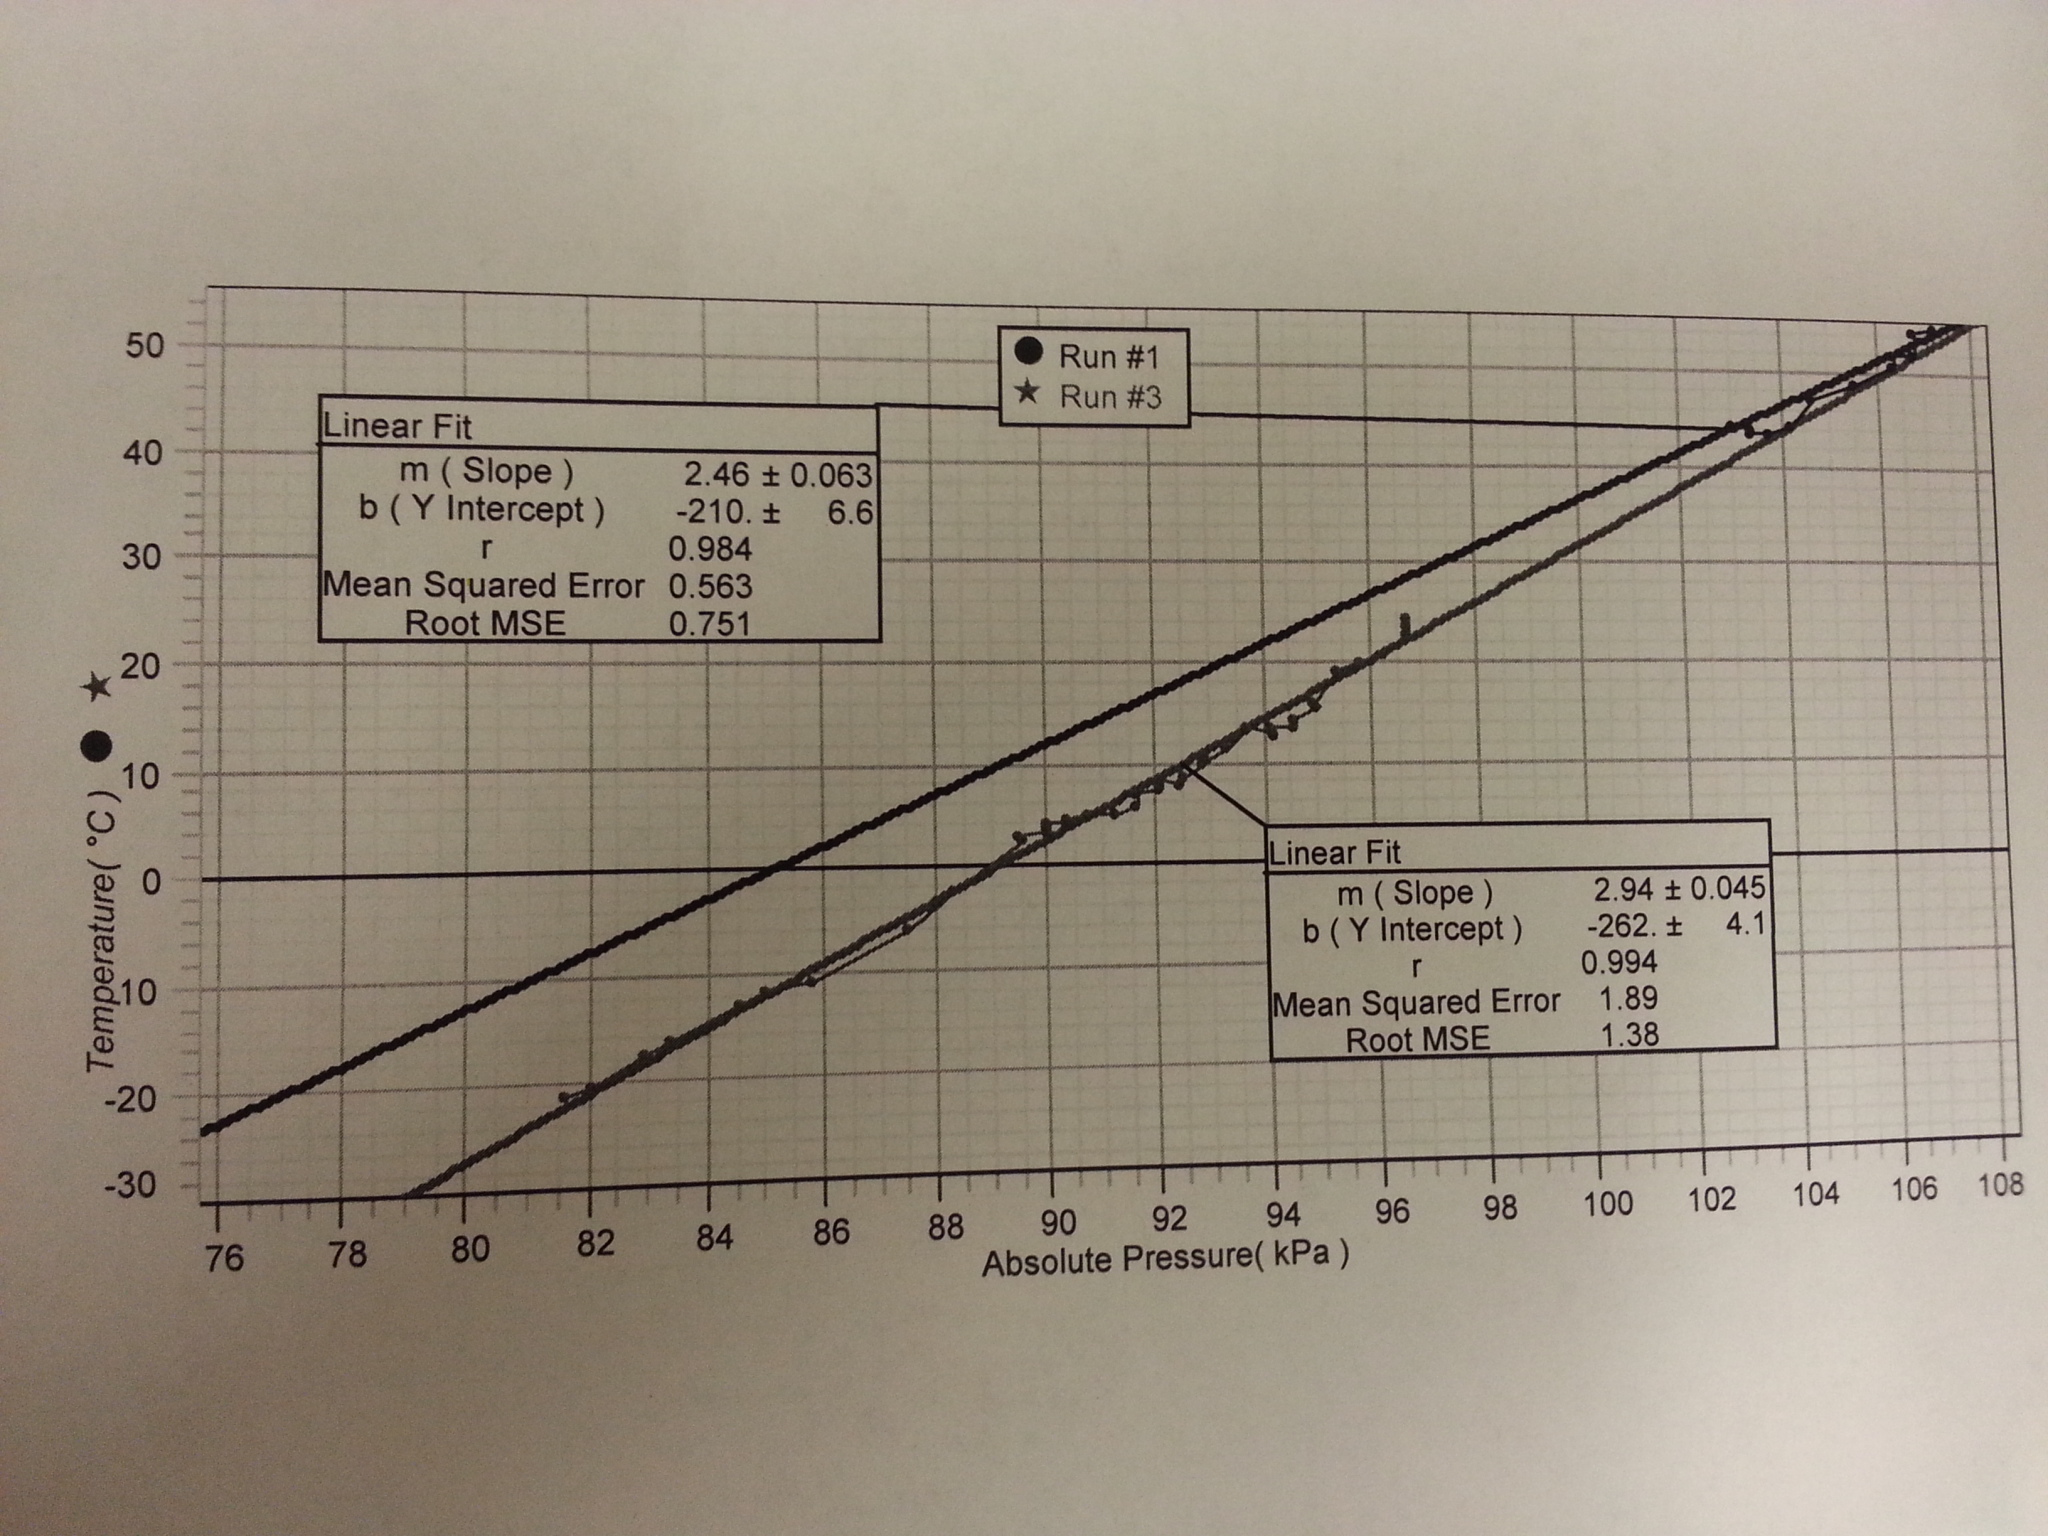
\includegraphics[scale=0.2]{both_graphs}
Above, is the image of both of my measurements as graphs from both parts of the experiment.\\
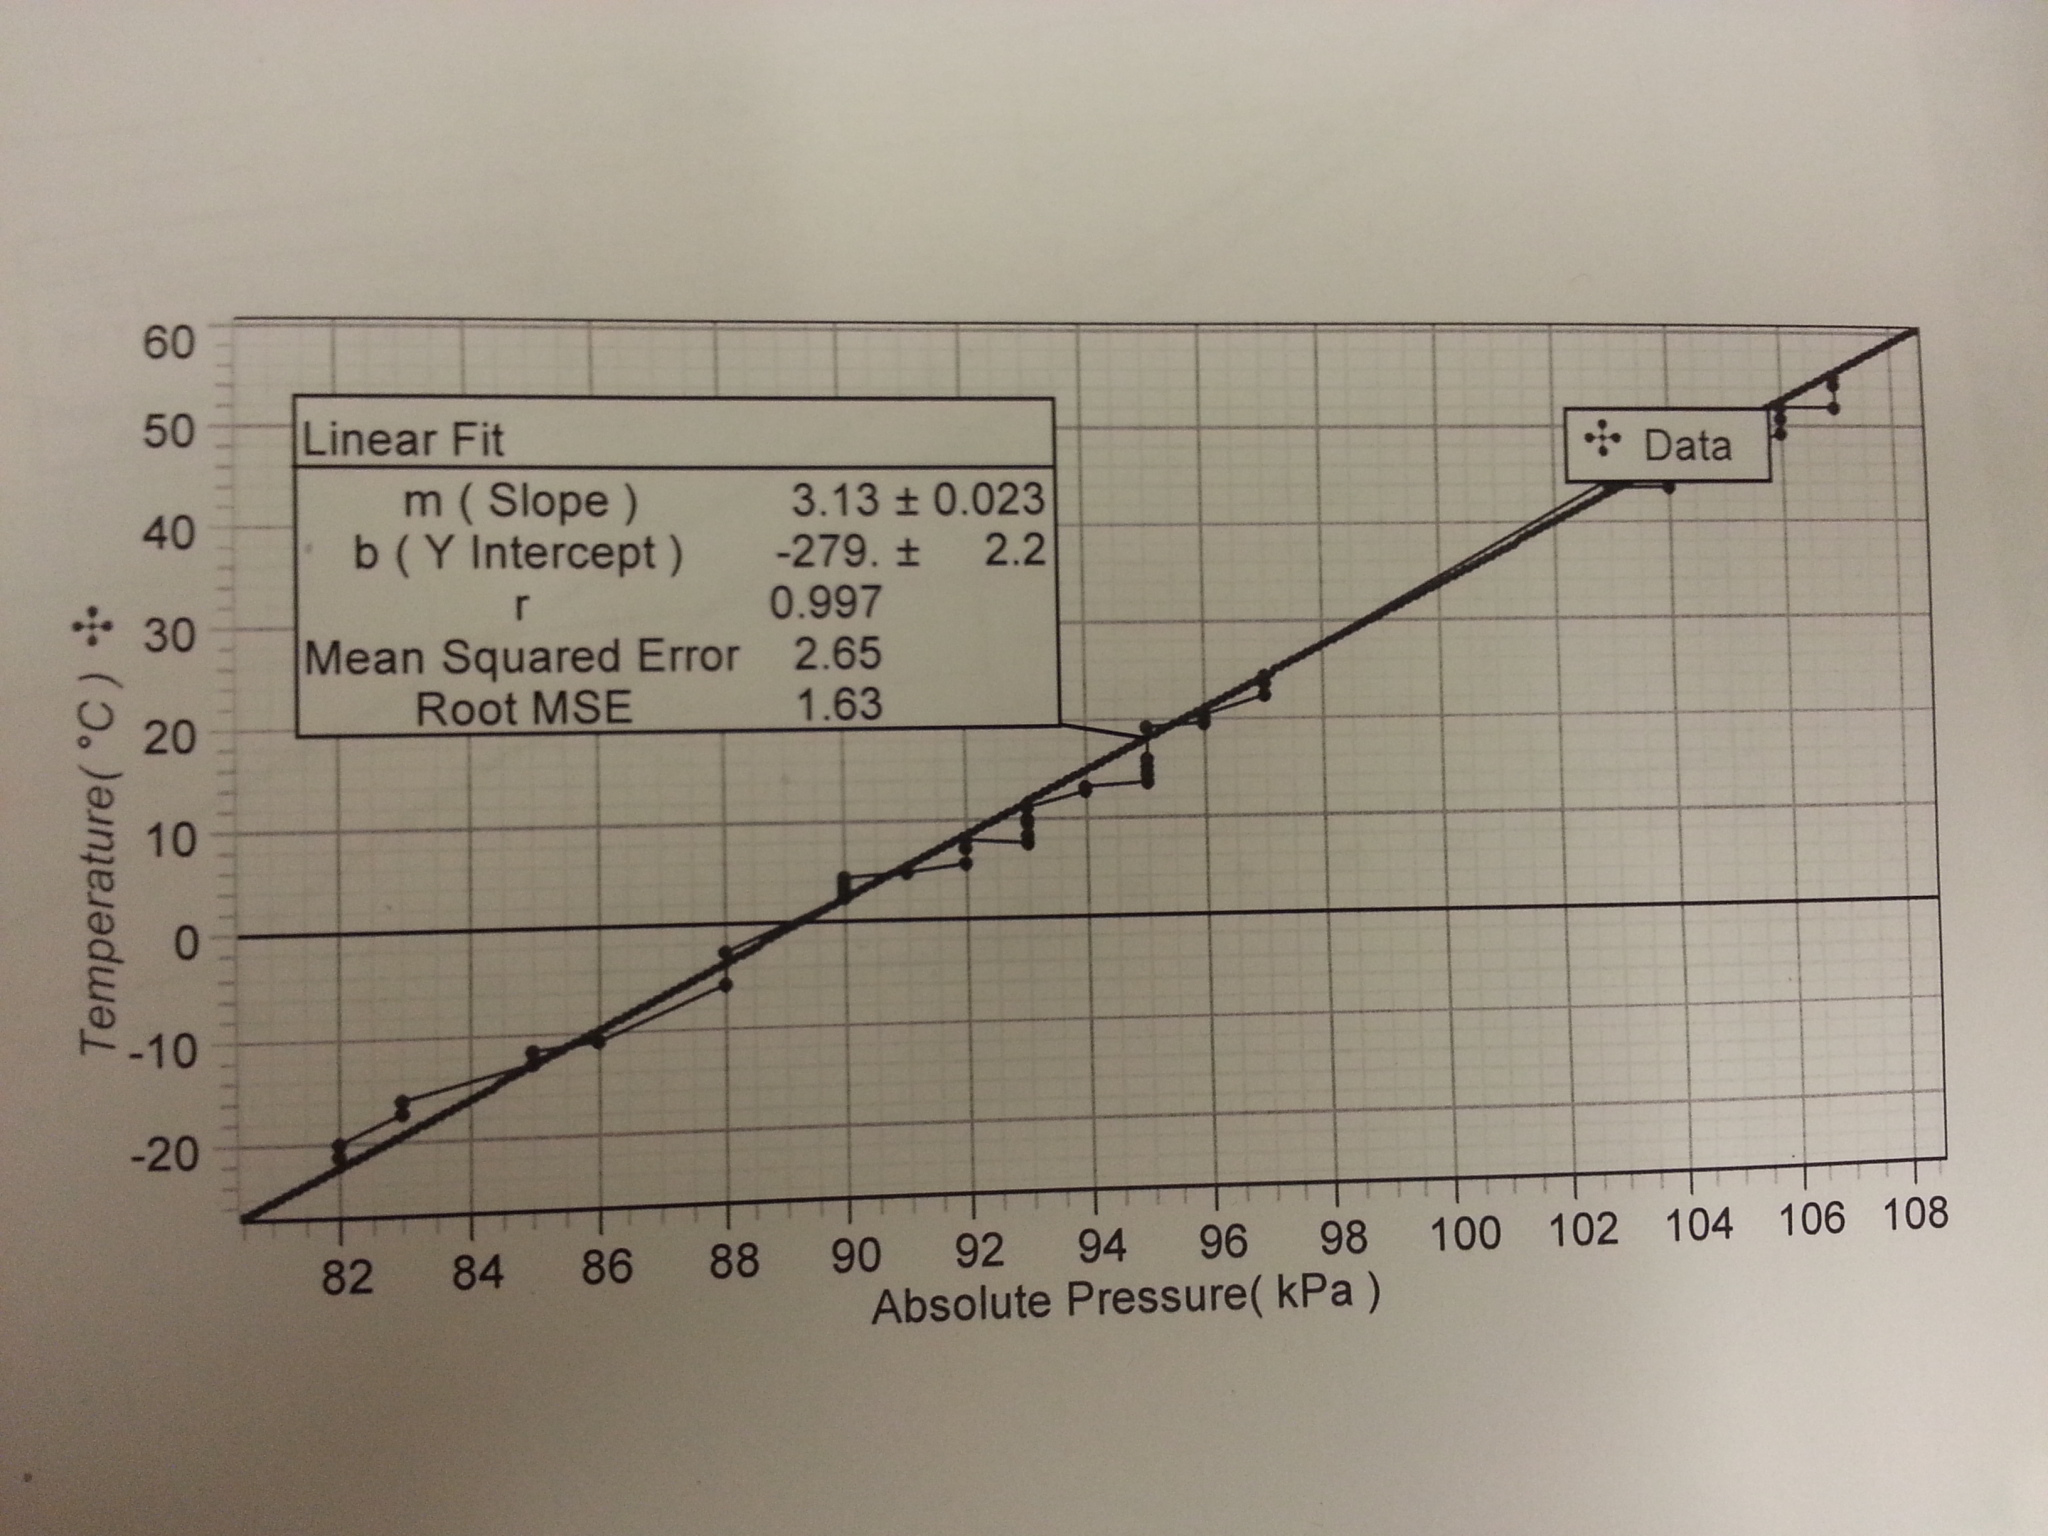
\includegraphics[scale=0.2]{OverallGraphs}
Above is the image of the overall graph of both parts of the experiment.
Both of these pictures are for number 4.
\end{document}